\begin{figure}
    \begin{center}
        \begin{adjustbox}{width=0.4\textwidth}

            \tikzset{every picture/.style={line width=0.75pt}} %set default line width to 0.75pt        
            
            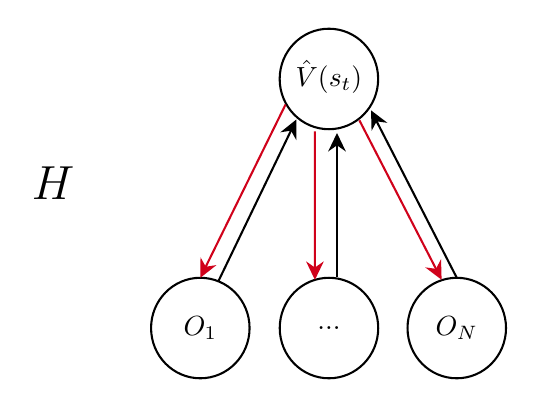
\begin{tikzpicture}[x=0.75pt,y=0.75pt,yscale=-1,xscale=1]
            %uncomment if require: \path (0,488); %set diagram left start at 0, and has height of 488
            
            %Shape: Ellipse [id:dp7350394708339132] 
            \draw   (292.58,215.46) .. controls (292.58,202.09) and (303.2,191.25) .. (316.3,191.25) .. controls (329.41,191.25) and (340.03,202.09) .. (340.03,215.46) .. controls (340.03,228.83) and (329.41,239.67) .. (316.3,239.67) .. controls (303.2,239.67) and (292.58,228.83) .. (292.58,215.46) -- cycle ;
            %Shape: Ellipse [id:dp360084071411103] 
            \draw   (230.62,335.46) .. controls (230.62,322.09) and (241.24,311.25) .. (254.35,311.25) .. controls (267.45,311.25) and (278.07,322.09) .. (278.07,335.46) .. controls (278.07,348.83) and (267.45,359.67) .. (254.35,359.67) .. controls (241.24,359.67) and (230.62,348.83) .. (230.62,335.46) -- cycle ;
            %Shape: Ellipse [id:dp6910252330291001] 
            \draw   (292.61,335.46) .. controls (292.61,322.09) and (303.23,311.25) .. (316.33,311.25) .. controls (329.44,311.25) and (340.06,322.09) .. (340.06,335.46) .. controls (340.06,348.83) and (329.44,359.67) .. (316.33,359.67) .. controls (303.23,359.67) and (292.61,348.83) .. (292.61,335.46) -- cycle ;
            %Shape: Ellipse [id:dp08711921105296772] 
            \draw   (354.18,335.46) .. controls (354.18,322.09) and (364.8,311.25) .. (377.91,311.25) .. controls (391.01,311.25) and (401.63,322.09) .. (401.63,335.46) .. controls (401.63,348.83) and (391.01,359.67) .. (377.91,359.67) .. controls (364.8,359.67) and (354.18,348.83) .. (354.18,335.46) -- cycle ;
            %Straight Lines [id:da1085527921907381] 
            \draw [color={rgb, 255:red, 208; green, 2; blue, 27 }  ,draw opacity=1 ]   (255.67,308.55) -- (295.4,227.8) ;
            \draw [shift={(254.35,311.25)}, rotate = 296.2] [fill={rgb, 255:red, 208; green, 2; blue, 27 }  ,fill opacity=1 ][line width=0.08]  [draw opacity=0] (8.93,-4.29) -- (0,0) -- (8.93,4.29) -- (5.93,0) -- cycle    ;
            %Straight Lines [id:da2379350098727664] 
            \draw [color={rgb, 255:red, 208; green, 2; blue, 27 }  ,draw opacity=1 ]   (309.56,309.25) -- (309.53,240.67) ;
            \draw [shift={(309.56,312.25)}, rotate = 269.98] [fill={rgb, 255:red, 208; green, 2; blue, 27 }  ,fill opacity=1 ][line width=0.08]  [draw opacity=0] (8.93,-4.29) -- (0,0) -- (8.93,4.29) -- (5.93,0) -- cycle    ;
            %Straight Lines [id:da04155200209198706] 
            \draw [color={rgb, 255:red, 0; green, 0; blue, 0 }  ,draw opacity=1 ]   (320.2,244.5) -- (320.2,311) ;
            \draw [shift={(320.2,241.5)}, rotate = 90] [fill={rgb, 255:red, 0; green, 0; blue, 0 }  ,fill opacity=1 ][line width=0.08]  [draw opacity=0] (8.93,-4.29) -- (0,0) -- (8.93,4.29) -- (5.93,0) -- cycle    ;
            %Straight Lines [id:da5357018140104348] 
            \draw [color={rgb, 255:red, 0; green, 0; blue, 0 }  ,draw opacity=1 ]   (299.3,237.7) -- (263,313) ;
            \draw [shift={(300.6,235)}, rotate = 115.74] [fill={rgb, 255:red, 0; green, 0; blue, 0 }  ,fill opacity=1 ][line width=0.08]  [draw opacity=0] (8.93,-4.29) -- (0,0) -- (8.93,4.29) -- (5.93,0) -- cycle    ;
            %Straight Lines [id:da1804092882370092] 
            \draw [color={rgb, 255:red, 208; green, 2; blue, 27 }  ,draw opacity=1 ]   (369.23,309.53) -- (331,235.4) ;
            \draw [shift={(370.6,312.2)}, rotate = 242.72] [fill={rgb, 255:red, 208; green, 2; blue, 27 }  ,fill opacity=1 ][line width=0.08]  [draw opacity=0] (8.93,-4.29) -- (0,0) -- (8.93,4.29) -- (5.93,0) -- cycle    ;
            %Straight Lines [id:da17854416312427956] 
            \draw [color={rgb, 255:red, 0; green, 0; blue, 0 }  ,draw opacity=1 ]   (337.97,233.27) -- (377.91,311.25) ;
            \draw [shift={(336.6,230.6)}, rotate = 62.88] [fill={rgb, 255:red, 0; green, 0; blue, 0 }  ,fill opacity=1 ][line width=0.08]  [draw opacity=0] (8.93,-4.29) -- (0,0) -- (8.93,4.29) -- (5.93,0) -- cycle    ;
            
            % Text Node
            \draw (316.33,214.5) node   [align=left] {$\displaystyle \hat{V}( s_{t})$};
            % Text Node
            \draw (171.67,256.4) node [anchor=north west][inner sep=0.75pt]  [font=\LARGE]  {$H$};
            % Text Node
            \draw (254.35,335.46) node   [align=left] {$\displaystyle O_{1}$};
            % Text Node
            \draw (316.33,335.46) node   [align=left] {$\displaystyle ...$};
            % Text Node
            \draw (377.91,335.46) node   [align=left] {$\displaystyle O_{N}$};
            \end{tikzpicture}
        \end{adjustbox}
    \end{center}
\caption[\textbf{Diagram of a Global Model}]{The figure represents how multiple $O$ can simultaneously contribute to the estimation of $\widehat{V}(s_t)$. Here $\{O_1, \dots, O_N\}$ indicate a set of object on which the ANN is simultaneously fit. Black and red arrows are respectively the direction of the computations and the flow of the error gradient. Circles indicate computational blocks similar to those in figures \ref{fig: ffnn} and \ref{fig: ffnn_rnn}.}
\label{fig: global_model}
\end{figure}